
\documentclass[a4paper,12pt]{article}

\usepackage{graphicx} % Required for inserting images
\usepackage{amsmath,amssymb,amsfonts}
\usepackage{subcaption}
% -----------------------
% Package Imports
% -----------------------

% Set page margins
\usepackage[a4paper, top=1in, bottom=0.8in, left=1.1in, right=0.8in]{geometry}

% Use Times New Roman font
\usepackage{times}

% Add page numbering
\pagestyle{plain}

% Enable graphics inclusion
\usepackage{graphicx}
\usepackage{float}
% Enable code listings
\usepackage{listings}
\usepackage{xcolor} % For customizing code colors
\setlength{\parindent}{0pt}


% -----------------------
% Document Content
% -----------------------

\begin{document}
	
	% -----------------------
	% Title Page
	% -----------------------
	%\begin{titlepage}
	
	
	
	
	% -----------------------
	% Table of Contents (Optional)
	% -----------------------
	%\tableofcontents
	\newpage
	
	% -----------------------
	% Sections
	% -----------------------
	\section{Experiment No. 1}
	
	\section{Experiment Title }
	Introduction to the Construction and Operation of DC Motors, DC Generators, and Transformers
	
	
	% Objective Section
	\section{Objective}
	The main objectives of this report are:
	\begin{itemize}
		\item To provide an introduction to DC machines, focusing on DC motors, DC generators, and transformers.
		\item To explain the fundamental construction and working principles of DC machines.
		\item To highlight the differences in the construction and operation between DC motors, generators, and transformers.
		\item To discuss the significance of these machines in modern electrical systems and their applications in various industries.
	\end{itemize}
	
	
	% Theory Section
	\section{Theory}
	DC machines, including DC motors, generators, and transformers, are fundamental components in various electrical systems. The construction of these machines typically includes key components such as the stator, rotor, commutator, and windings.
	
	\subsection{DC Motor}
	
	
	A DC motor is a type of electric motor that converts direct current (DC) electrical energy into mechanical energy. It works on the principle of electromagnetism, where a current-carrying conductor, placed in a magnetic field, experiences a force. This force creates rotation in the motor, which is used to drive mechanical systems.\\
	\subsubsection{Construction of DC Motor}
	A DC motor converts electrical energy into mechanical energy. The basic construction of a DC motor consists of:
	\begin{enumerate}\item \textbf{Stator (Field Poles):}  
		The stationary part of the motor, providing a magnetic field via electromagnets or permanent magnets.
		
		\item \textbf{Rotor (Armature):}  
		The rotating part of the motor, made of laminated steel with copper windings that generate torque when interacting with the stator’s magnetic field.
		
		\begin{figure}[h]
			\centering
			\includegraphics[width=0.6\linewidth]{"Images/DC MOTOR"}
			\caption[Construction of DC Motor]{Construction of DC Motor}
			\label{fig:dc-motor}
		\end{figure}
		
		\item \textbf{Commutator:}  
		A segmented cylinder attached to the rotor, reversing current direction in the armature windings for continuous rotation.
		
		\item \textbf{Brushes:}  
		Carbon or graphite elements that transfer current between the stationary and rotating parts, maintaining contact with the commutator.
		
		\item \textbf{Shaft:}  
		Transfers the rotor’s mechanical energy to external loads like gears or wheels.
		
		\item \textbf{Yoke (Frame):}  
		Provides mechanical support and completes the magnetic path between poles and armature.
		
		\item \textbf{Field Windings:}  
		Coils wound around poles to generate the magnetic field needed for motor operation.
		
		\item \textbf{Armature Windings:}  
		Copper coils in the rotor slots, creating torque through interaction with the magnetic field.
		
		\item \textbf{Bearings:}  
		Reduce friction between the rotating shaft and the motor housing for smooth operation.
		
		\item \textbf{Pole Core and Pole Shoes:}  
		Attached to the yoke, supporting field windings and distributing the magnetic field evenly over the armature.
		
	\end{enumerate}
	
	 \subsubsection{Working Process of a DC Motor}
	 \begin{figure}[h]
	 	\centering
	 	
	 	\begin{subfigure}[t]{0.49\textwidth}
	 		\centering
	 		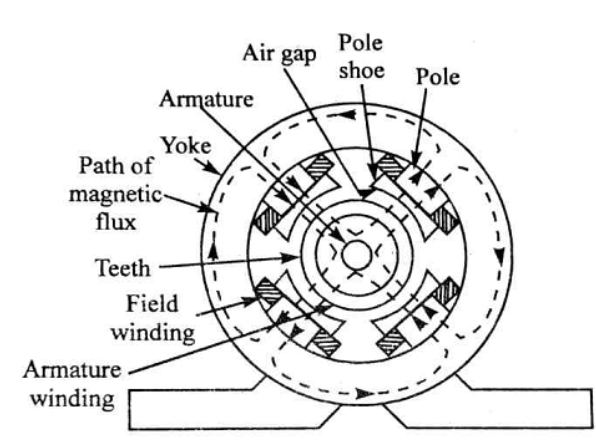
\includegraphics[width=1\textwidth , height=.25\textheight]{Images/2D VIEW}
	 		\caption{2D View of DC Motor}
	 		\label{fig:3-a}
	 	\end{subfigure}
	 	\hfill
	 	\begin{subfigure}[t]{0.49\textwidth}
	 		\centering
	 		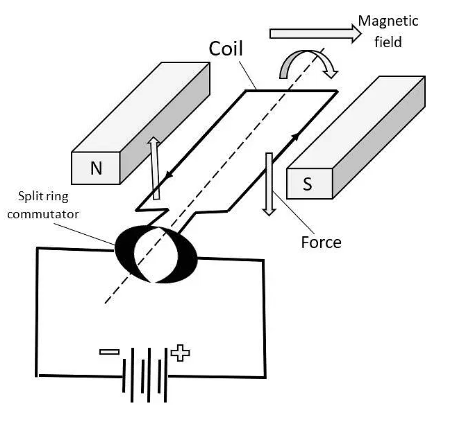
\includegraphics[width=1\textwidth, height=0.25\textheight]{Images/working proocess DC MOTOR}
	 		\caption{Working process of DC Motor}
	 		\label{fig:3-b}
	 	\end{subfigure}
	 	\caption{ Working process of DC Motor}
	 	\label{fig:3}
	 \end{figure}
	 
	The working process of a DC motor can be broken down into the following steps:
	
	\begin{enumerate}
		\item \textbf{Current Flow:} When a direct current (DC) is applied to the motor terminals, it flows through the brushes and the commutator into the armature windings.
		
		\item \textbf{Magnetic Field Interaction:} The current flowing through the armature windings generates an electromagnetic force, which interacts with the magnetic field produced by the stator (either permanent magnets or electromagnets).
		
		\item \textbf{Torque Generation:} According to **Fleming’s Left-Hand Rule**, the interaction between the magnetic field and the current generates a force on the armature. This force produces a torque, which causes the armature (rotor) to rotate.
		
		\item \textbf{Commutator Action:} The commutator segments ensure that the current direction in the armature windings reverses each time the armature rotates by 180 degrees. This reversal ensures that the torque acting on the armature remains in the same direction, allowing continuous rotation.
		
		\item \textbf{Shaft Rotation:} The rotating armature turns the motor shaft, which is attached to the external load. This converts the electrical energy supplied to the motor into mechanical energy (rotational motion).
		
		\item \textbf{Energy Transfer:} As the motor continues to rotate, the mechanical energy generated is transferred to an external device, such as a fan or conveyor belt.
	\end{enumerate}
	

	% DC Machine Specifications
	\subsubsection{DC Motor Specifications}
	\begin{table}[H]
		\centering
		\caption{DC Motor Specifications}
		\begin{tabular}{| c | c |}
			\hline
			\textbf{Specification} & \textbf{Value} \\ \hline
			Power Rating & 300 W\\ \hline
			Voltage Rating [EXC.SERIES \& EXC. SEP] & 220 V \\ \hline
			Current Rating [EXC SERIES] & 1.9 A \\ \hline
			Current Rating [EXC SEP] & 1.8 A \\ \hline
			Vexc & 220 V \\ \hline
			Iexc & 0.1 A \\ \hline
			Speed & 2500 RPM \\ \hline
			
		\end{tabular}
		
		
		\label{tab:2}
	\end{table}
	
	
	\subsection{DC Generator}
	A DC generator is an electrical machine that converts mechanical energy into direct current (DC) electrical energy. It operates on the principle of electromagnetic induction, where a conductor moving through a magnetic field induces an electric current. The primary components of a DC generator include a stator, which provides the magnetic field, and a rotor or armature, where the electrical current is generated. The generated voltage is then collected using a commutator, which converts the alternating current (AC) generated in the armature into direct current for external circuits.\\
	
	\subsubsection[short title]{Construction of a DC Generator}
A DC generator consists of several key components that work together to convert mechanical energy into electrical energy. Below is a detailed description of the main parts:
\begin{figure}[h]
	\centering
	\includegraphics[width=0.5\linewidth]{"Images/DC Generator"}
	\caption[DC Generator]{DC Generator}
	\label{fig:dc-generator}
\end{figure}

	\begin{enumerate}
\item \textbf{Yoke (Frame):} 
The outer frame of the generator, providing mechanical support, protecting internal components, and serving as a path for magnetic flux. It is made of cast iron or steel.

\item \textbf{Field Poles and Windings:} 
Mounted on the yoke, the field poles generate the magnetic field. Each pole has a winding (field coil) that, when energized, produces the necessary magnetic flux.

\item \textbf{Armature Core:} 
The rotating part of the generator, made of laminated soft iron to reduce core losses. It holds the armature windings and provides a low-reluctance path for magnetic flux.

\item \textbf{Armature Windings:} 
Located in the slots of the armature core, these windings carry the current. When the armature rotates within the magnetic field, an EMF is induced, generating power.

\item \textbf{Commutator:} 
A mechanical rectifier that converts AC to DC, consisting of copper segments insulated by mica. It reverses the current direction to produce a unidirectional output.

\item \textbf{Brushes:} 
Made of carbon or graphite, brushes transfer current from the rotating armature to the external circuit. They maintain contact with the commutator segments.

\item \textbf{Shaft:} 
The rotating part to which the armature is attached, converting mechanical energy into electrical energy.

\item \textbf{Bearings:} 
Installed at the ends of the shaft, bearings reduce friction and support the loads during operation.

	\end{enumerate}
	\subsubsection{Working Process of a DC Generator}
	
	The working principle of a DC generator is based on Faraday's law of electromagnetic induction, which states that an electromotive force (EMF) is induced in a conductor when it moves in a magnetic field. Here's a brief overview of the working process:
		\begin{enumerate}
	\item \textbf{Magnetic Field Creation:}	 The field windings, attached to the field poles, are excited by an external DC supply, producing a magnetic field in the generator.
		
	\item \textbf{Armature Rotation:}		 Mechanical energy, often from a turbine or motor, rotates the armature core inside the magnetic field.
		
		\item \textbf{Induced EMF:}	 As the armature windings (conductors) rotate within the magnetic field, the flux linkage with the conductors changes, inducing an electromotive force (EMF) according to Faraday's law.
		
		\item \textbf{Current Flow:}	 The induced EMF causes a current to flow through the armature windings. The direction of the current alternates with each half-turn of the armature.
		
		\item \textbf{Commutation: }	The commutator reverses the direction of the current flow in the windings, converting the alternating current (AC) generated in the armature into direct current (DC) for external use.
		
		\item \textbf{Output:}	 The carbon brushes collect the current from the rotating commutator and deliver it to the external load, providing DC power.
		
		\end{enumerate}
	
	This process converts mechanical energy into electrical energy in the form of direct current.
	
	% DC Generator Specifications
	\subsubsection{DC Generator Specifications}
	\begin{table}[H]
		\centering
			\caption{DC Generator}
		\begin{tabular}{| c | c |}
			\hline
			\textbf{Specification} & \textbf{Value} \\ \hline
			Power Rating & 300 W\\ \hline
			Voltage Rating [EXC.SERIES] & 210 V \\ \hline
			Voltage Rating [ EXC. COMP] & 220 V \\ \hline
			Current Rating [EXC SERIES \& EXC COMP] & 1.4 A \\ \hline
			Vexc & 0-220 V \\ \hline
			Iexc & 0.11 A \\ \hline
			Speed & 3000 RPM \\ \hline
			
		\end{tabular}
	
		\label{tab:2}
	\end{table}
	
	
	
	
	
	\subsection{Transformer}
	A transformer is a device that transfers electrical energy between two or more circuits through electromagnetic induction. It typically consists of:
	\begin{itemize}
		\item \textbf{Primary Coil:} Receives the input voltage and creates a magnetic field.
		\item \textbf{Secondary Coil:} Receives the induced voltage from the primary coil’s magnetic field.
		\item \textbf{Core:} Provides a path for the magnetic flux, enhancing efficiency.
	\end{itemize}
\subsubsection{Single-Phase Transformer}
\begin{figure}[h]
	\centering
	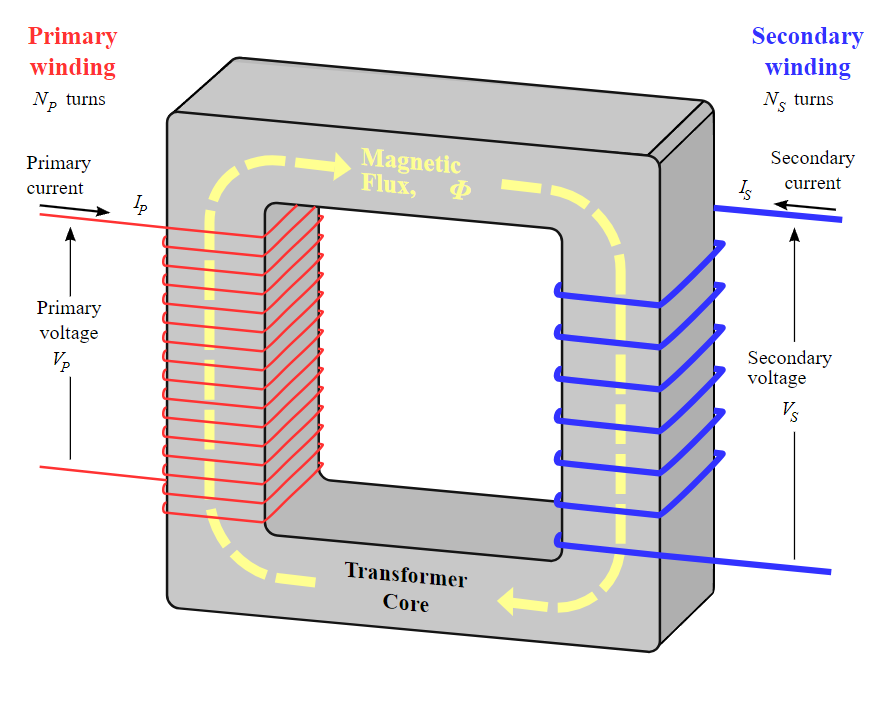
\includegraphics[width=0.5\linewidth]{Images/T1}
	\caption[Single Phase Transformer]{Single Phase Transformer}
	\label{fig:t1}
\end{figure}

A single-phase transformer is designed to operate on a single-phase power supply. It consists of two windings: the primary and secondary windings, each with a specific number of turns. These transformers are commonly used in household applications, such as in appliances and lighting, where the power supply is single-phase (e.g., 120V or 240V). They are simpler in construction and are suitable for low-power applications\\[0.2cm]
\textbf{	Single-Phase Transformer Construction:}
\begin{enumerate}
\item \textbf{Core: }
The core is typically made of laminated sheets of steel to minimize eddy current losses. It serves as the path for the magnetic flux generated by the primary winding.
\item \textbf{Primary Winding:}  The primary winding is the coil connected to the input voltage source. It generates the magnetic field when an alternating current flows through it.
\item \textbf{Secondary Winding }: The secondary winding is connected to the load, where the transformed (stepped-up or stepped-down) voltage is delivered. Both the primary and secondary windings are wound around the same core but are electrically isolated.
\item \textbf{Insulation:}  The windings are insulated from each other and the core to prevent electrical contact and short circuits.
\item \textbf{Tank(for larger transformers):}   Larger single-phase transformers may have a tank containing cooling oil to dissipate heat generated during operation.
\end{enumerate}

\subsubsection{Single-Phase Transformer Specifications}
\begin{table}[H]
	\centering
	\caption{Single-Phase Transformer Specifications}
	\begin{tabular}{| c |c |}
		\hline
		\textbf{Specification} & \textbf{Value} \\ \hline
		Power Rating & 760 kVA \\ \hline
		$U_1$  & 230 V \\ \hline
		$U_2$  & 400V-230V \\ \hline
		$I_1$ & 3.7 A \\ \hline
		$I_2$ & 1A-1.7A \\ \hline
		Frequency & 50 Hz \\ \hline
		
	\end{tabular}
	
	
	\label{tab:3}
\end{table}


	\subsubsection{Three-Phase Transformer}
	A three-phase transformer is designed to work with three-phase power, which is used in industrial and large-scale electrical systems. It consists of three sets of windings, one for each phase. Three-phase transformers are more efficient and capable of handling larger loads compared to single-phase transformers. They are commonly used in power distribution, industrial machinery, and large electric motors.\\[.2cm]
	\textbf{Three-Phase Transformer Construction:}
	 \begin{figure}[h]
		\centering
		
		\begin{subfigure}[t]{0.49\textwidth}
			\centering
			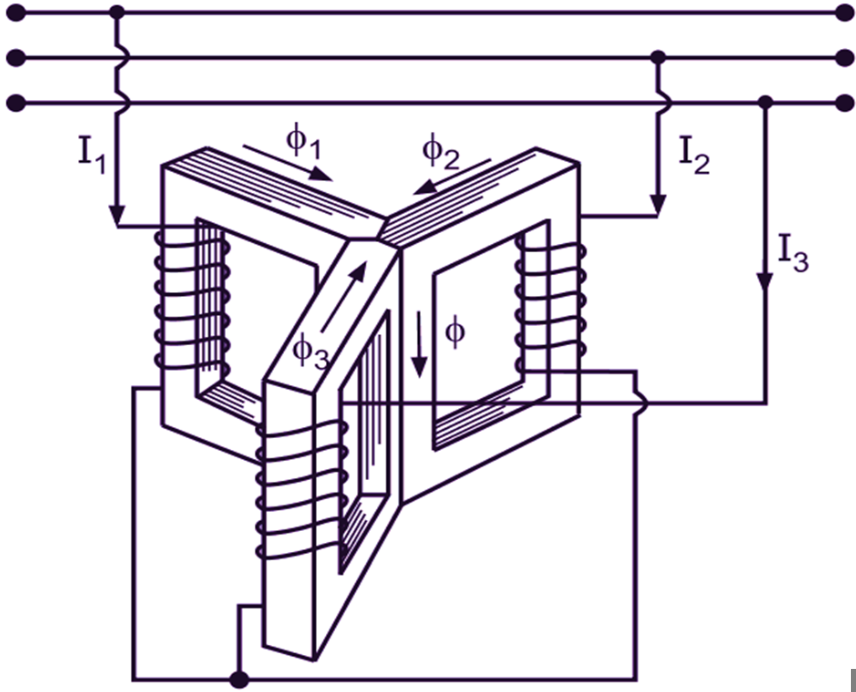
\includegraphics[width=1\textwidth , height=.25\textheight]{Images/T3}
			\caption{Simplified View}
			\label{fig:3-a}
		\end{subfigure}
		\hfill
		\begin{subfigure}[t]{0.49\textwidth}
			\centering
			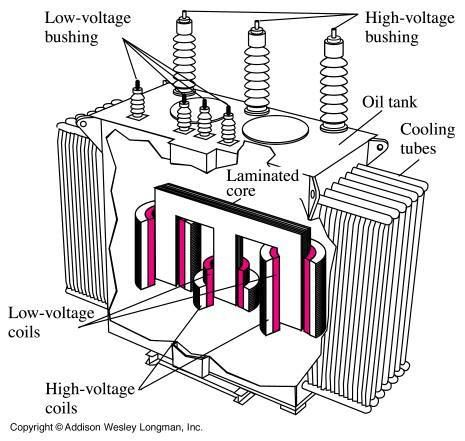
\includegraphics[width=1\textwidth, height=0.25\textheight]{Images/T3.2}
			\caption{Three Phase Transformer Parts}
			\label{fig:3-b}
		\end{subfigure}
		\caption{Three Phase Transformer}
		\label{fig:3}
	\end{figure}
	

	\begin{enumerate}
		\item \textbf{Core:}  The core in a three-phase transformer is usually of laminated steel, just like in single-phase transformers. It can have three or five limbs depending on the design, with the three limbs corresponding to the three phases.
	\item \textbf{	Windings:} Each phase in a three-phase transformer has a primary and a secondary winding. These windings are distributed across the limbs of the core.
	\item \textbf{	Primary Windings:} Connected to the input three-phase power supply.
		\item \textbf{Windings:}Secondary  Delivers the transformed three-phase voltage to the load.
	\item \textbf{Winding Configuration:}	 The windings can be connected in different configurations, such as star $(Y)$ or delta  $\Delta$, depending on the application requirements.
	\item \textbf{Insulation:}	 As with single-phase transformers, the windings are insulated to avoid short circuits and electrical losses.
	\item \textbf{Tank and Cooling:}	 Due to the higher power capacity of three-phase transformers, they are typically housed in a tank filled with insulating oil for cooling. Radiators and fans may be included for additional cooling.
	\item \textbf{Bushings: }	These are used to connect external conductors to the windings through the transformer casing, ensuring safety and insulation.
	\end{enumerate}

	
\section{Conclusion}
This lab report has provided a detailed exploration of DC machines, including DC motors, DC generators, and both single-phase and three-phase transformers. These devices are fundamental to the conversion and management of electrical and mechanical energy in various systems.\\

DC motors and generators are essential for converting electrical energy into mechanical energy, and vice versa, which makes them critical in industrial and commercial applications. Additionally, the study of single-phase and three-phase transformers has demonstrated their importance in efficiently transferring electrical energy across varying voltage levels. These transformers are key components in power distribution systems, ensuring reliable energy flow in residential, commercial, and industrial environments.\\

By understanding the construction and operation of these machines, we gain valuable insights into the field of electrical engineering. This foundational knowledge not only strengthens our grasp of existing technologies but also prepares us for future advancements and innovations in electrical machines and power systems.


	
	
	
	
\end{document}
